\documentclass{article}
\usepackage[utf8]{inputenc}
\usepackage{geometry}
\usepackage{booktabs}   % For nicer tables
\usepackage{array}      % For table arrays
\usepackage{listings}   % For SQL code formatting
\usepackage{xcolor}     % For colors
\usepackage{tikz}       % For drawing diagrams
\usetikzlibrary{shapes.geometric, arrows, positioning, shapes.multipart}

% Page Margins
\geometry{a4paper, margin=1in}

% SQL Code Style Setup
\definecolor{codegreen}{rgb}{0,0.6,0}
\definecolor{codegray}{rgb}{0.5,0.5,0.5}
\definecolor{codepurple}{rgb}{0.58,0,0.82}
\definecolor{backcolour}{rgb}{0.95,0.95,0.92}

\lstdefinestyle{mystyle}{
    backgroundcolor=\color{backcolour},   
    commentstyle=\color{codegreen},
    keywordstyle=\color{magenta},
    numberstyle=\tiny\color{codegray},
    stringstyle=\color{codepurple},
    basicstyle=\ttfamily\footnotesize,
    breakatwhitespace=false,         
    breaklines=true,                 
    captionpos=b,                    
    keepspaces=true,                 
    numbers=left,                    
    numbersep=5pt,                  
    showspaces=false,                
    showstringspaces=false,
    showtabs=false,                  
    tabsize=2
}
\lstset{style=mystyle}

% Define block styles for Schema Diagram
\tikzset{
    entity/.style={
        draw, 
        rectangle split, 
        rectangle split parts=2, 
        text centered, 
        text width=4cm, 
        minimum height=1cm,
        fill=blue!10
    },
    line/.style={
        draw, -latex'
    }
}

\title{\textbf{Lab 5 Assignment: DBMS (CS264)}\\ \large Project: Pharmacy E-Commerce System}
\author{Name: [Your Name Here] \\ ID: [Your ID Here] \\ Batch/Section: [Your Section]}
\date{\today}

\begin{document}

\maketitle

\section*{Project Overview}
\textbf{Topic:} Pharmacy E-Commerce (Medicine Marketplace)\\
\textbf{Description:} A system allowing Customers to order Medicines from various Shops (Pharmacies). The system tracks inventory, orders, and shop details.

\hrule
\vspace{0.5cm}

% ==========================================
% SECTION 1
% ==========================================
\section{Section 1: Functional Dependencies & Keys}

\subsection{1. Functional Dependencies (FDs)}
Based on the project requirements, the following Functional Dependencies satisfy the business logic:

\begin{itemize}
    \item \textbf{FD1 (Customer):} $cust\_id \rightarrow \{name, phone, address\}$
    \item \textbf{FD2 (Shop):} $shop\_id \rightarrow \{shop\_name, location, owner\}$
    \item \textbf{FD3 (Medicine):} $med\_id \rightarrow \{med\_name, mfg, price\}$
    \item \textbf{FD4 (Inventory):} $\{shop\_id, med\_id\} \rightarrow \{stock\_qty\}$
    \item \textbf{FD5 (Orders):} $order\_id \rightarrow \{cust\_id, shop\_id, med\_id, date, amount\}$
\end{itemize}

\subsection{2. Minimal Canonical Cover}
The Minimal Canonical Cover is the set of dependencies where no redundancy exists. Since our design is already normalized, the canonical cover is simply the decomposed version of the FDs above:
\begin{itemize}
    \item $cust\_id \rightarrow name$, $cust\_id \rightarrow phone$
    \item $shop\_id \rightarrow shop\_name$, $shop\_id \rightarrow location$
    \item $med\_id \rightarrow med\_name$, $med\_id \rightarrow price$
    \item $\{shop\_id, med\_id\} \rightarrow stock\_qty$
\end{itemize}

\subsection{3. Candidate Keys}
The unique identifiers for each relation are:
\begin{itemize}
    \item \textbf{Customer:} $cust\_id$
    \item \textbf{Shop:} $shop\_id$
    \item \textbf{Medicine:} $med\_id$
    \item \textbf{Inventory:} $\{shop\_id, med\_id\}$ (Composite Key)
    \item \textbf{Orders:} $order\_id$
\end{itemize}

\newpage

% ==========================================
% SECTION 2
% ==========================================
\section{Section 2: Schema Design \& Implementation}

\subsection{1. Database Schema Diagram}
Below is the visual representation of the tables and their attributes.
\vspace{0.5cm}

\begin{center}
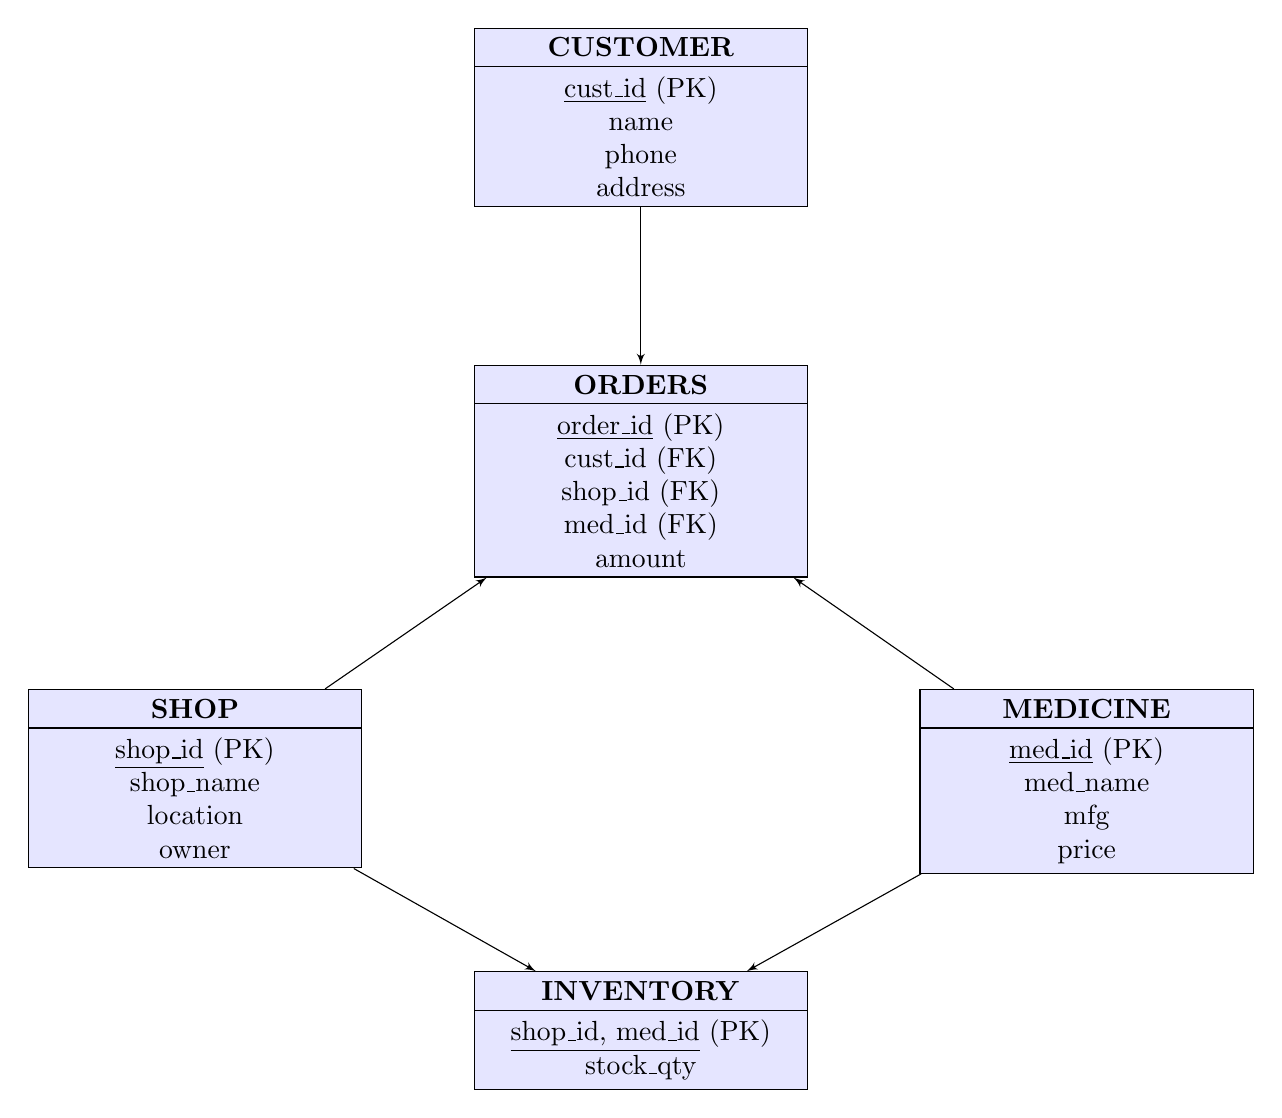
\begin{tikzpicture}[node distance=2cm]

% Customer Table
\node (cust) [entity] {
    \textbf{CUSTOMER}
    \nodepart{second}
    \underline{cust\_id} (PK)\\
    name\\
    phone\\
    address
};

% Order Table
\node (order) [entity, below=of cust] {
    \textbf{ORDERS}
    \nodepart{second}
    \underline{order\_id} (PK)\\
    cust\_id (FK)\\
    shop\_id (FK)\\
    med\_id (FK)\\
    amount
};

% Shop Table
\node (shop) [entity, below left=of order] {
    \textbf{SHOP}
    \nodepart{second}
    \underline{shop\_id} (PK)\\
    shop\_name\\
    location\\
    owner
};

% Medicine Table
\node (med) [entity, below right=of order] {
    \textbf{MEDICINE}
    \nodepart{second}
    \underline{med\_id} (PK)\\
    med\_name\\
    mfg\\
    price
};

% Inventory Table
\node (inv) [entity, below=of order, yshift=-3cm] {
    \textbf{INVENTORY}
    \nodepart{second}
    \underline{shop\_id, med\_id} (PK)\\
    stock\_qty
};

% Relationships (Lines)
\draw[line] (cust) -- (order);
\draw[line] (shop) -- (order);
\draw[line] (med) -- (order);
\draw[line] (shop) -- (inv);
\draw[line] (med) -- (inv);

\end{tikzpicture}
\end{center}

\vspace{0.5cm}
\textbf{Note:} Arrows indicate Foreign Key relationships (e.g., Orders references Customer).

\newpage

\subsection{2. SQL Create Statements}
The following SQL commands create the tables with Primary Keys (PK) and Foreign Keys (FK).

\begin{lstlisting}[language=SQL, caption=Database Creation Scripts]
-- 1. Customer Table
CREATE TABLE Customer (
    cust_id INT PRIMARY KEY,
    name VARCHAR(50),
    phone VARCHAR(15),
    address VARCHAR(100)
);

-- 2. Shop Table (Retailers)
CREATE TABLE Shop (
    shop_id INT PRIMARY KEY,
    shop_name VARCHAR(50),
    location VARCHAR(50),
    owner VARCHAR(50)
);

-- 3. Medicine Table (Product Catalog)
CREATE TABLE Medicine (
    med_id INT PRIMARY KEY,
    med_name VARCHAR(50),
    mfg VARCHAR(50),
    price DECIMAL(10, 2)
);

-- 4. Inventory Table (Many-to-Many Link)
CREATE TABLE Inventory (
    shop_id INT,
    med_id INT,
    stock_qty INT,
    PRIMARY KEY (shop_id, med_id),
    FOREIGN KEY (shop_id) REFERENCES Shop(shop_id),
    FOREIGN KEY (med_id) REFERENCES Medicine(med_id)
);

-- 5. Orders Table
CREATE TABLE Orders (
    order_id INT PRIMARY KEY,
    cust_id INT,
    shop_id INT,
    med_id INT,
    amount DECIMAL(10, 2),
    FOREIGN KEY (cust_id) REFERENCES Customer(cust_id),
    FOREIGN KEY (shop_id) REFERENCES Shop(shop_id),
    FOREIGN KEY (med_id) REFERENCES Medicine(med_id)
);
\end{lstlisting}

\subsection{3. Normalization Analysis}

\textbf{1NF (First Normal Form):}
All attributes contain atomic values. There are no repeating groups or multi-valued attributes (e.g., the 'phone' column contains only one number).

\textbf{2NF (Second Normal Form):}
The schema is in 2NF because there are no partial dependencies. 
\begin{itemize}
    \item In the \textbf{Inventory} table (which has a composite key $\{shop\_id, med\_id\}$), the non-key attribute $stock\_qty$ depends on the \textit{entire} key, not just part of it.
    \item All other tables have single-column primary keys, so 2NF is automatically satisfied.
\end{itemize}

\textbf{3NF (Third Normal Form) \& BCNF:}
The schema is in 3NF and BCNF because there are no transitive dependencies. 
\begin{itemize}
    \item Non-key attributes depend \textbf{only} on the Primary Key. 
    \item For example, in the \textbf{Medicine} table, $manufacturer$ depends directly on $med\_id$, not on $med\_name$.
\end{itemize}

\end{document}